\documentclass[twocolumn]{article}
\setlength{\oddsidemargin}{-0.1875in}
\setlength{\evensidemargin}{-0.1875in}
\setlength{\columnsep}{0.3125in}
\setlength{\topmargin}{-0.75in}
\setlength{\textheight}{8.875in}
\setlength{\textwidth}{6.875in}
\setlength{\headheight}{0.3in}
\setlength{\marginparwidth}{.7in}
\setcounter{topnumber}{2}
\setcounter{bottomnumber}{2}
\renewcommand{\topfraction}{1.0}
\renewcommand{\bottomfraction}{1.0}
\renewcommand{\textfraction}{.00}
\setcounter{totalnumber}{4}

%\setlength{\floatsep}{0pt plus 2pt minus 2pt}
\setlength{\textfloatsep}{4pt plus 2pt minus 4pt}

\usepackage{amssymb}
\usepackage{amstext}
\usepackage{array}
\usepackage{boxedminipage}
\usepackage{calc}
\usepackage{citesort}
\usepackage[dvips]{epsfig}
\usepackage{fancybox}
\usepackage{fancyheadings}
\usepackage{fleqn}
\usepackage{hhline}
\usepackage{multirow}
\usepackage{psboxit}
\usepackage{pst-node}
\usepackage{pstricks}
\usepackage{stretch}
\usepackage{subfigure}
\usepackage{theorem}
\usepackage{times}
\usepackage{timestamp}
\usepackage{verbatim}
\usepackage{xspace}

\PScommands

\setlength{\mathindent}{0in}

\renewcommand{\baselinestretch}{1.0}
\newcommand{\eg}{e.g.,\xspace}
\newcommand{\ie}{i.e.,\xspace}
\newcommand{\etc}{etc.\@\xspace}
\makeatletter
\newcommand{\preprint}
    {\pagestyle{empty}
     \newcommand{\firstpage}
         {\thispagestyle{plain}
          \makeatletter
          \renewcommand{\ps@plain}{
              \renewcommand{\@oddhead}{\fbox{To appear in \textit{Proceedings
                                             11th International Conference on
                                             Data Engineering},
                                             Taipei, March 1995}}
              \renewcommand{\@evenhead}{}
              \renewcommand{\@evenfoot}{}
              \renewcommand{\@oddfoot}{}}
          \makeatother}}
\newcommand{\reprint}
    {\pagestyle{empty}
     \newcommand{\firstpage}
         {\thispagestyle{plain}
          \makeatletter
          \renewcommand{\ps@plain}{
              \renewcommand{\@oddhead}{\fbox{In \textit{Proceedings
                                             11th International Conference on
                                             Data Engineering}, pages 201--210,
                                             Taipei, March 1995}}
              \renewcommand{\@evenhead}{}
              \renewcommand{\@evenfoot}{}
              \renewcommand{\@oddfoot}{}}
          \makeatother}}
\makeatother
\newcommand{\final}
    {\pagestyle{empty}
     \newcommand{\firstpage}{\thispagestyle{empty}}}
\newcommand{\myshadowsize}{2pt}
\newcommand{\myshadowbox}{\setlength{\shadowsize}{\myshadowsize}\shadowbox}
\newcommand{\doubleopenbraces}{\{\{}
\newcommand{\doubleclosebraces}{\}\}}
\newcommand{\nodesizes}{\scriptsize}
\newlength{\edgesizes}
\setlength{\edgesizes}{6mm}
\newcommand{\graybox}[3]{\psboxit{box .5 setgray fill}{\makebox[#1][#2]{#3}}}

\theoremstyle{plain}
\theoremheaderfont{\scshape}
\theorembodyfont{\rmfamily}
\newtheorem{myexample}{Example}
\renewcommand{\themyexample}{\arabic{myexample}.}
\newenvironment{example}
    {\begin{myexample}\quad}
    {\hfill$\Box$\end{myexample}}
\newenvironment{smalleqnarray*}[1]
    {#1
     \begin{eqnarray*}}
    {\end{eqnarray*}
     \normalsize}

\newenvironment{quarterminipage}
    {\begin{minipage}[b]{0.22\linewidth}}
    {\end{minipage}}
\newenvironment{halfminipage}
    {\begin{minipage}[b]{0.44\linewidth}}
    {\end{minipage}}
\newenvironment{fullminipage}
    {\begin{minipage}[b]{0.93\linewidth}}
    {\end{minipage}}

\newenvironment{fullminipagerule}
    {\setlength{\topsep}{0pt}
     \scriptsize
     \begin{fullminipage}}
    {\end{fullminipage}}
\newenvironment{halfminipagerule}
    {\setlength{\topsep}{0pt}
     \footnotesize
     \begin{halfminipage}}
    {\end{halfminipage}}

% Command to add space to second line of rule definitions.
\newcommand{\rulespace}{\quad}
\newenvironment{ruleactions}
    {$\doubleopenbraces$
     \begin{tabbing}
     \hspace{2pc} \= \kill}
    {\end{tabbing}
     $\doubleclosebraces$}

\newenvironment{trule}
    {\begin{equation}}
    {\end{equation}}
\newenvironment{trulepretest}
    {\begin{ruleactions}}
    {\end{ruleactions} \\}
\newenvironment{truleposttest}
    {\\
     \begin{ruleactions}}
    {\end{ruleactions}}
\newenvironment{fullminipagetrule}
    {\begin{fullminipagerule}}
    {\end{fullminipagerule}}
\newenvironment{halfminipagetrule}
    {\begin{halfminipagerule}}
    {\end{halfminipagerule}}

\newenvironment{irule}
    {\begin{equation}}
    {\end{equation}}
\newenvironment{irulepreopt}
    {\\
     \begin{ruleactions}}
    {\end{ruleactions}}
\newenvironment{irulepostopt}
    {\\
     \begin{ruleactions}}
    {\end{ruleactions}}
\newenvironment{fullminipageirule}
    {\begin{fullminipagerule}}
    {\end{fullminipagerule}}
\newenvironment{halfminipageirule}
    {\begin{halfminipagerule}}
    {\end{halfminipagerule}}

\newenvironment{centeredfigure}
    {\begin{figure}[tb]
     \begin{center}}
    {\end{center}
     \end{figure}}
\newenvironment{centeredfigure*}
    {\begin{figure*}[tb]
     \begin{center}}
    {\end{center}
     \end{figure*}}

\newenvironment{centeredtable}
    {\begin{table}[tb]
     \begin{center}}
    {\end{center}
     \normalsize
     \end{table}}
\newenvironment{centeredtable*}
    {\begin{table*}[tb]
     \begin{center}}
    {\end{center}
     \normalsize
     \end{table*}}

\newenvironment{centeredinquarterminipage}
    {\begin{quarterminipage}
     \begin{center}}
    {\end{center}
     \end{quarterminipage}}
\newenvironment{centeredinhalfminipage}
    {\begin{halfminipage}
     \begin{center}}
    {\end{center}
     \end{halfminipage}}
\newenvironment{centeredinfullminipage}
    {\begin{fullminipage}
     \begin{center}}
    {\end{center}
     \end{fullminipage}}

\title{\textbf{Prairie: A Rule Specification Framework \\
       for Query Optimizers}\thanks{
       This research was supported in part by grants from The University
       of Texas Applied Research Laboratories, Schlumberger, and
       Digital Equipment Corporation.}\ \thanks{
       An expanded version of this paper is available as Technical
       Report TR 94--16 by anonymous ftp from \texttt{ftp.cs.utexas.edu}.}}
\author{Dinesh Das \hspace{1in} Don Batory \\
        Department of Computer Sciences \\
        The University of Texas at Austin \\
        Austin, Texas 78712--1188 \\
        \{ddas,batory\}@cs.utexas.edu}
\date{}

%\final
%\preprint
\reprint

\makeatletter
\def\thickhline{\noalign{\ifnum0=`}\fi\hrule \@height 1.5pt \futurelet
   \@tempa\@xhline}
\makeatother

\begin{document}

\maketitle

\pagenumbering{arabic}
%%% abstract
%%% ---------------------------------------------------------------------------
\begingroup

%%% english
%%% ...........................................................................
\addchap{Abstract}

\blindtext


%%% german
%%% ...........................................................................
\otherlanguage{ngerman}
\addchap{Kurzfassung}

\blindtext

\endgroup
\chapter{The introduction}
Modern research on lexical access began in the 1950's (though
\cite{ColeRudnicky1983} note very similar research performed in the 1890's by
William Chandler Bagley).  Several statistical properties of the mental
lexicon have consistently been found to influence how humans process speech.
One of the earliest and most robust findings was that lexical frequency has a
strong influence on lexical access. Repeated research has shown that high
frequency words elicit quicker and more accurate responses than low
frequency words in a large variety of experimental conditions
(e.g.\ \cite{Broadbent1967, Taft1979, BenkiJASA}). Another factor which has
been reliably shown to affect lexical access is neighborhood density.
Neighborhood density is a metric of similarity, roughly defined as the degree
to which a word is similar to others (both phonological and orthographical
measures have been used). Words which have many similar words are said to be
in dense neighborhoods, whereas words which have few similar words are said to
be in sparse neighborhoods. In contrast to lexical frequency, which
facilitates the activation of a word in the brain, neighborhood density has
been found to inhibit activation (e.g.\ \cite{Luce1986, Luce1998, BenkiJASA,
Imai2005}). Of course these are not the only factors which affect language
processing, but they are the most frequently cited, and will be referred to
again in the following sections.
\begin{table*}[!htb]
  \centering
  \caption[Basic Predictions]{Basic Predictions: Predicted results are marked
  with a checkmark, and a relative effect size is also given.}
  \label{T:predictions}
  \begin{tabularx}{\textwidth}{%
    >{\setlength{\hsize}{1.5\hsize}\raggedright\arraybackslash}X%
    *{2}{>{\setlength{\hsize}{.7\hsize}\raggedright\arraybackslash}X}%
    *{2}{>{\setlength{\hsize}{1.05\hsize}\raggedright\arraybackslash}X}}
  \hline\hline
  \rule{0em}{1.1em}& English native listeners& German native listeners & 
       English non-native listeners & German non-native listeners\\[.3em]
  \cline{2-5}
  \rule{0em}{1.1em}lexical status & \checkmark robust& \checkmark
  robust& \checkmark less than native listeners& \checkmark less than native
  listeners\\
  morphology & marginal & more than English & less than L1& less than L1\\
  lexical frequency & \checkmark robust& \checkmark
  robust& \checkmark less than native listeners& \checkmark less than native
  listeners\\
  neighborhood density & \checkmark robust & \checkmark robust & \checkmark less
  than L1& \checkmark less than L1\\[.3em]
  \hline\hline
  \end{tabularx}
\end{table*}

\section{Prairie: A language for rule specification}
\label{sec:framework}

The basic concepts and definitions that underlie the Prairie model are
presented in this section.  The goal is to lay a foundation for
reasoning about query optimization algebraically; this is necessary for
our subsequent discussion about translating Prairie specifications to
those of Volcano.

\subsection {Notation and assumptions}
\label{sec:notation}

\paragraph{Stored Files and Streams.}
A file is \emph{stored} if its tuples reside on disk.  In the case of
relational databases, stored files are sometimes called \emph{base
relations}; we will denote them by $R$ or $R_i$.  In object-oriented
schemas, stored files are \emph{classes}; we will denote them by
$\textit{C}$ or $\textit{C}_i$.  Henceforth, whenever we refer to a
stored file, we mean a relation or a class; when the distinction is
unimportant, we will use $F$ or $F_i$.  A \emph{stream} is a sequence
of tuples and is the result of a computation on one or more streams or
stored files; tuples of streams are returned one at a time, typically
on demand.  Streams can be \emph{named}, denoted by $S_i$, or
\emph{unnamed}.

\paragraph{Database Operations.}
An \emph{operation} is a computation on one or more streams or stored
files.  There are two types of database operations in Prairie:
abstract (or implementation-unspecified) operators and concrete
algorithms.  Each is detailed below.
\begin{description} % To achieve extra indentation.
\begin{description}
\item[Operators.]
Abstract (or conceptual) \emph{operators} specify computations on
streams or stored files; they are denoted by all capital
letters (\eg JOIN).  Operators have two types of parameters:
essential and additional.  \emph{Essential parameters} are the stream
or file inputs to an operator; these are the primary inputs to be
processed by an operator.   \emph{Additional parameters} are
``fine-grain'' qualifications of an operator; their purpose is to
describe an operator in more detail than essential parameters.

\item[Algorithms.]
\emph{Algorithms} are concrete implementations of conceptual operators;
they will be represented in lower case with the first letter
capitalized (\eg Nested\_loops).  Algorithms have at least the same
essential and additional parameters as the conceptual operators that
they implement.\footnote{Algorithms may have \emph{tuning parameters}
which are not parameters of the operators they implement.}
Furthermore, there can be, and usually are, several algorithms for a
particular operator.
\end{description}
\end{description}
Table~\ref{tab:operators} lists some operators and algorithms implementing
them together with their additional parameters.

\begin{centeredtable*}
\begin{minipage}[b]{9.9cm}
\nodesizes
\newlength{\first}
\settowidth{\first}{JOIN($S_1$, $S_2$)}
\newlength{\second}
\settowidth{\second}{Join streams $S_1$, $S_2$}
\newlength{\third}
\settowidth{\third}{projected\_attributes}
\newlength{\fourth}
\settowidth{\fourth}{Nested\_loops($S_1$, $S_2$)}
\newlength{\linelength}
\setlength{\linelength}{\fourth+\tabcolsep*2}
\begin{tabular}{|l|l|l|p{\fourth}|} \thickhline
\textbf{Operator}
    & \textbf{Description}
    & \textbf{Additional Parameters}
    & \textbf{Algorithm} \\ \thickhline
\multirow{2}{\first}{JOIN($S_1$, $S_2$)}
    & \multirow{2}{\second}{Join streams $S_1$, $S_2$} & tuple\_order
    & Nested\_loops($S_1$, $S_2$) \\ \cline{4-4}
  & & join\_predicate & Merge\_join($S_1$, $S_2$) \\ \hline
\multirow{3}{\first}{RET($F$)}
    & \multirow{3}{\second}{Retrieve file $F$}
    & tuple\_order
    & \parbox[c][\baselineskip][b]{\fourth}{File\_scan($F$)} \\
  & & selection\_predicate
    & \parbox[c]{\linelength}
                {\hspace*{-\tabcolsep}\rule{\linelength}{\arrayrulewidth}} \\ 
  & & projected\_attributes
    & \parbox[c][\baselineskip][t]{\fourth}{Index\_scan($F$)} \\ \hline
\multirow{2}{\first}{SORT($S_1$)}
    & \multirow{2}{\second}{Sort stream $S_1$}
    & \multirow{2}{\third}{tuple\_order}
    & Merge\_sort($S_1$) \\ \cline{4-4}
  & & & Null($S_1$) \\ \thickhline
\end{tabular}
\caption{Operators and algorithms in a centralized query optimizer and
         their additional parameters}
\label{tab:operators}
\end{minipage}
\hfill
\begin{minipage}[b]{6.5cm}
\nodesizes
\settowidth{\first}{projected\_attributes}
\begin{tabular}{|l|l|}  \thickhline
\textbf{Property} 
    & \textbf{Description} \\ \thickhline
join\_predicate
    & join predicate for JOIN operator \\ \hline
selection\_predicate
    & selection predicate for RET operator \\ \hline
\multirow{2}{\first}{tuple\_order}
    & tuple order of resulting stream, \\
    & DONT\_CARE if none \\ \hline
num\_records
    & number of tuples of resulting stream \\ \hline
tuple\_size
    & size of individual tuple in stream \\ \hline
projected\_attributes
    & projected attributes for RET operator \\ \hline
attributes
    & list of attributes \\ \hline
cost
    & estimated cost of algorithm \\ \thickhline
\end{tabular}
\caption{Properties of nodes in an operator tree}
\label{tab:annotations}
\end{minipage}
\end{centeredtable*}

\paragraph{Operator Trees.}
An \emph{operator tree} is a rooted tree whose non-leaf, or
\emph{interior}, nodes are database operations (operators or
algorithms) and whose leaf nodes are stored files.  The children of an
interior node in an operator tree are the essential parameters (\ie the
stream or file parameters) of the node.  Additional parameters are
implicitly attached to each node.  Algebraically, operator trees are
compositions of database operations; thus, we will also call operator
trees \emph{expressions}; both terms will be used interchangeably.

\begin{example}
A simple expression and its operator tree representation are shown
in Figure~\ref{fig:optreeexample}.  Relations $R_1$ and $R_2$ are first 
RETrieved, then JOINed, and finally SORTed resulting in a stream
sorted on a specific attribute.  The figure shows only the essential
parameters of the various operators, not the additional parameters.
\end{example}

\begin{comment}
The figures which follow.

               SORT
                 |
                 |
               JOIN
                /\
               /  \
             RET  RET
              |    |
              |    |
             R1   R2

            Merge_sort
                |
                |
           Nested_loops
               / \
              /   \
        File_scan File_scan
            |         |
            |         |
           R1        R2

\end{comment}

\begin{centeredfigure}
\setlength{\unitlength}{0.6in}
%
\myshadowbox
{
\subfigure[An expression and its corresponding operator tree]
{
\begin{centeredinhalfminipage}
\psset{unit=4mm}
\psset{nodesep=1pt}
\tiny
\begin{pspicture}(0,0)(2,4)
\rput(1,4){SORT (JOIN (RET ($R_1$), RET ($R_2$)))}
\rput(1,3){\rnode{sort}{SORT}}
\rput(1,2){\rnode{join}{JOIN}}
\ncline{-}{sort}{join}
\rput(0,1){\rnode{retr1}{RET}}
\rput(2,1){\rnode{retr2}{RET}}
\ncline{-}{join}{retr1}
\ncline{-}{join}{retr2}
\rput(0,0){\rnode{r1}{$R_1$}}
\rput(2,0){\rnode{r2}{$R_2$}}
\ncline{-}{retr1}{r1}
\ncline{-}{retr2}{r2}
\end{pspicture}
\end{centeredinhalfminipage}
\label{fig:optreeexample}
}
%
\vrule
%
\subfigure[Possible access plan for operator tree in (a)]
{
\begin{centeredinhalfminipage}
\psset{unit=4mm}
\psset{nodesep=1pt}
\tiny
\begin{pspicture}(0,0)(2,3)
\rput(1,3){\rnode{mergesort}{Merge\_sort}}
\rput(1,2){\rnode{nestedloops}{Nested\_loops}}
\ncline{-}{mergesort}{nestedloops}
\rput(0,1){\rnode{filescanr1}{File\_scan}}
\rput(2,1){\rnode{filescanr2}{File\_scan}}
\ncline{-}{nestedloops}{filescanr1}
\ncline{-}{nestedloops}{filescanr2}
\rput(0,0){\rnode{r1}{$R_1$}}
\rput(2,0){\rnode{r2}{$R_2$}}
\ncline{-}{filescanr1}{r1}
\ncline{-}{filescanr2}{r2}
\end{pspicture}
\end{centeredinhalfminipage}
\label{fig:accplanexample}
}
}
%
\caption{Example of an operator tree and access plan}
\label{fig:expexample}
\end{centeredfigure}

\paragraph{Descriptors.}
A \emph{property} of a node is a (user-defined) variable that contains
information used by an optimizer.  An \emph{annotation} is a $\langle
\emph{property, value} \rangle$ pair that is assigned to a node.  A
\emph{descriptor} is a list of annotations that describes a node of an
operator tree; every node has its own descriptor.  As an example,
Table~\ref{tab:annotations} lists some typical properties that might be
used in a descriptor.  Note that descriptors for stream and stored
files may have different properties.  The following notations will be
useful in our subsequent discussions.  If $S_i$ is a stream, then
$\mathbf{D_i}$ is its descriptor.  Annotations of $S_i$ are accessed by
a structure member relationship, \eg
$\mathbf{D_i}.\text{num\_records}$.  Also, let $E$ be an expression and
let $\mathbf{D}$ be its descriptor.  We will write this as
$E:\mathbf{D}$.

\begin{example}
The expression,
\begin{eqnarray*}
{\scriptstyle \text{SORT}(\text{JOIN}(\text{RET}(R_1):\mathbf{D_3},
      \text{RET}(R_2):\mathbf{D_4}):\mathbf{D_5}):\mathbf{D_6}} & &
\end{eqnarray*}
corresponds to the operator tree in Figure~\ref{fig:optreeexample}, and
shows the descriptors of the various nodes.
\end{example}

A notational simplification can be made here.  Additional parameters
of operators can be treated the same way as other properties of a node;
essential parameters, however, are \emph{expressions}.  Thus, the term
descriptor in the remainder of this paper will refer to a set of properties,
including additional parameters, as shown in Table~\ref{tab:annotations}.

Currently, descriptor properties are defined entirely by the user;
however, we envision providing a hierarchy of pre-defined descriptor
types to aid this process.

\paragraph{Access Plans.}
An \emph{access plan} is an operator tree in which all interior nodes
are algorithms.

\begin{example}
An access plan for the operator tree in Figure~\ref{fig:optreeexample}
is shown in Figure~\ref{fig:accplanexample}.
\end{example}

\subsection{Prairie optimization paradigm}
\label{sec:topdown}

Prairie admits two rather different means of optimization: top-down and
bottom-up.  A top-down query optimizer optimizes the parents of a node
prior to optimizing the node itself.  A bottom-up optimizer optimizes
the children of a node prior to optimizing the node.  The earliest
optimizers (System R \cite{Seli79} and R$^*$ \cite{Dani82}) employed
the bottom-up approach.

Our research concentrates on a top-down optimization of operator
trees.  We have chosen this approach because we intend to translate
Prairie rules into the format required by the Volcano query optimizer
generator \cite{Grae90b} which is based on a top-down strategy.
Given an appropriate search engine, Prairie can potentially also be
used with a bottom-up optimization strategy; however, we will not
discuss this approach in this paper.

In query optimization, there are certain annotations (such as
additional parameters) that are known before any optimization is
begun.  These annotations can be computed at the time that the operator
tree is initialized, and will not change with application of rules.
Our following discussions assume operator trees are initialized.

There are two types of algebraic transformations (or \emph{rewrite
rules}) in Prairie: T-rules (``transformation rules'') and I-rules
(``implementation rules'').  Each rule transforms an expression into
another based on additional conditions; the transformation also results
in a mapping of descriptors between expressions.  We define T-rules and
I-rules precisely in the following sections and illustrate them with
examples.  Our examples are chosen from rules that would be used in a
centralized relational query optimizer; the operators, algorithms, and
properties are subsets of those in Tables~\ref{tab:operators} and
\ref{tab:annotations}.

\subsection{Transformation rules}
\label{sec:trules}

\begin{centeredfigure}
\def\subfigtopskip{0pt}
\myshadowbox{
\begin{tabular}{c}
\subfigure[General form of a T-rule]
{
\setlength{\topsep}{0pt}
\scriptsize
\begin{minipage}[b]{0.86\linewidth}
\begin{trule}
E(x_1, \ldots, x_n):\mathbf{D_1} \Longrightarrow
        E'(x_1, \ldots, x_n):\mathbf{D_2} \label{eq:generaltrule}
\end{trule}
\begin{trulepretest}
\> pre-test statements
\end{trulepretest}
test
\begin{truleposttest}
\> post-test statements
\end{truleposttest}
\end{minipage}
\label{fig:generaltrule}
} \\ \hline
%%%
\subfigure[Join associativity]
{
\setlength{\topsep}{0pt}
\scriptsize
\begin{minipage}[b]{0.86\linewidth}
\vspace*{4pt}
\begin{trule}
\text{JOIN}(\text{JOIN}(S_1, S_2):\mathbf{D_4}, S_3):\mathbf{D_5}
\label{eq:associativity}
\end{trule}
%%% TODO: Remove extra space above eqnarray.
\begin{eqnarray*}
\rulespace \Longrightarrow
    \text{JOIN}(S_1, \text{JOIN}(S_2, S_3):\mathbf{D_6}):\mathbf{D_7}
%                                              \label{eq:associativity}
\end{eqnarray*}
\begin{trulepretest}
\> $\mathbf{D_6}.\text{attributes} =
     \text{union}\ (\mathbf{D_2}.\text{attributes},
                    \mathbf{D_3}.\text{attributes})\ ;$
\end{trulepretest}
$\text{is\_associative}\ (\mathbf{D_6}.\text{join\_predicate},
                             \mathbf{D_6}.\text{attributes},
                             \mathbf{D_5}.\text{join\_predicate})$
\begin{truleposttest}
\> $\mathbf{D_7} = \mathbf{D_5}\ ;$ \\
\> $\mathbf{D_7}.\text{join\_predicate} =
     \mathbf{D_4}.\text{join\_predicate}\ ;$ \\
\> $\mathbf{D_6}.\text{tuple\_size} =
     \mathbf{D_2}.\text{tuple\_size}
      + \mathbf{D_3}.\text{tuple\_size}\ ;$ \\
\> $\mathbf{D_6}.\text{num\_records} =
     \text{cardinality}\ (\mathbf{D_2}, \mathbf{D_3})\ ;$
\end{truleposttest}
\end{minipage}
\label{fig:associativity}
}
\end{tabular}
}
\caption{T-rule}
\label{fig:trules}
\end{centeredfigure}

Transformation rules, or T-rules for short, define equivalences among
pairs of expressions; they define mappings from one operator tree to
another.  Let $E$ and $E'$ be expressions that involve only abstract
operators.  Equation~(\ref{eq:generaltrule}) (shown in
Figure~\ref{fig:generaltrule}) shows the general form of a T-rule.  The
actions of a T-rule define the equivalences between the descriptors of
nodes of the original operator tree $E$ with the nodes of the output
tree $E'$; these actions consist of a series of (C or C++)
assignment\footnote{The actions can be non-assignment statements (like
function calls), but in this case, the P2V pre-processor (described in
Section~\ref{sec:ptov}) needs some hints about the properties that
are changed by the statement in order to correctly categorize each
property.  For simplicity, in this paper, we assume all actions consist
of assignment statements.} statements.  The left-hand sides of these
statements refer to descriptors of expressions on the right-hand side
of the T-rule; the right-hand sides of the statements can refer to any
descriptor in the T-rule.  Function (called \emph{helper} functions)
calls can also appear on the right side of the assignment statements.
Thus, descriptors on the \emph{left-hand side} of a T-rule are
\emph{never} changed in the rule's actions.  A \emph{test} is needed to
determine if the transformations of the T-rule are in fact applicable.

Purely as an optimization, it is usually the case that not all
statements in a T-rule's actions need to be executed prior to a
T-rule's test.  For this reason, the actions of a T-rule are split into
two groups; those that need to be executed prior to the T-rule's test,
and those that can be executed after a successful test.  These groups
of statements comprise, respectively, the \emph{pre-test} and
\emph{post-test} statements of the T-rule.\footnote{We suspect it is
possible to use data-flow analysis to partition the assignment
statements automatically, but for now, we let the rule-writer do the
partitioning.}

\begin{comment}
We now define the actions and tests of a T-rule more precisely.  Let
$O_i$ be an abstract operator of $E'$, and let $\mathbf{O_i}$ be its
descriptor.  Similarly, let $I_i$ be an abstract operator of $E$ and
let $\mathbf{I_i}$ be its descriptor. ($I_i$ is an operator that is
input to the rule and $O_i$ is an operator that is output by the
rule).  Let $M_i$ denote the $i$th descriptor property.  Thus,
$\mathbf{O_i}.M_j$ is the value of the $j$th property of descriptor
$\mathbf{O_i}$.  We have found that actions of a T-rule are invariably
assignment statements, since actions compute assignments to descriptor
properties.  Rather than admitting all possible computations, we will
present our model in terms of assignment statements.\footnote{ The
actions can be non-assignment statements (like function calls), but in
this case, the P2V pre-processor (described in
Section~\ref{sec:results}) needs some hints about the properties that
are changed by the statement in order to correctly categorize each
property.  For simplicity, in this paper, we assume all actions consist
of assignment statements.  } The left-hand side of an assignment refers
to an output descriptor ($\mathbf{O_i}$) or a member of an output
descriptor ($\mathbf{O_i}.M_j$).  The right-hand side is an expression
or function that only references input descriptors and/or their
members.  (We call such functions \emph{helper} functions; they are
defined externally to a rule).  Here are a few examples:
\[
\begin{array}{rlll}
\mathbf{O_i} & = & \mathbf{I_k}\ ; &
    \text{$//$ copy descriptor $\mathbf{I_k}$ to $\mathbf{O_i}$} \nonumber \\
\mathbf{O_i}.M_j & = & \mathbf{I_k}.M_j + 4\ ; &
    \text{$//$ expression defining $\mathbf{O_i}.M_j$} \nonumber \\
\mathbf{O_3}.M_5 & = & \text{helper}\ (\mathbf{I_1}.M_5, \mathbf{I_2}.M_5)\ ; &
    \text{$//$ helper function that computes $\mathbf{O_3}.M_5$} \nonumber \\
& & &
    \text{$//$ from inputs $\mathbf{I_1}.M_5$ and $\mathbf{I_2}.M_5$.} \nonumber
\end{array}
\]

The test for a T-rule's applicability is a boolean expression and
normally involves checks on the values of output descriptors (\eg
$\mathbf{O_3}.M_5 > 6$); occasionally, helper functions may be needed.

Again, it is important to remember that the pre-test actions are
carried out prior to the test; the post-test actions are performed only
if a T-rule's test evaluates to TRUE, and all post-test actions are
performed immediately, with no intermediate optimization of any
descendant nodes of the root of $E$.

Note that there are no actions that are carried out \emph{after} the
essential parameters of the root of $E$ are optimized.  This is because
a T-rule only logically transforms a conceptual tree into another
conceptual tree.
\end{comment}

\begin{example}
\label{ex:joinassociativity}
The associativity of JOINs is expressed by T-rule
(\ref{eq:associativity}) in Figure~\ref{fig:associativity}.
\end{example}

\begin{comment}

          b2=c1 JOIN                          JOIN a1=b1
                 /\                            /\
                /  \                          /  \
       a1=b1 JOIN  RET                      RET JOIN b2=c1
              /\    |        ====>          |    /\
             /  \  R3                      R1   /  \
           RET  RET                           RET  RET
            |    |                             |    |
           R1   R2                            R2   R3

          a2=c1 JOIN                           JOIN a1=b1
                 /\                             /\
                /  \                           /  \
       a1=b1 JOIN   RET                      RET  JOIN <empty>
              /\     |        ==/==>          |    /\
             /  \   R3                       R1   /  \
           RET  RET                             RET  RET
            |    |                               |    |
           R1   R2                              R2   R3

\end{comment}

\newsavebox{\lefttreeone}
\newsavebox{\righttreeone}
\newsavebox{\lefttreetwo}
\newsavebox{\righttreetwo}
\newsavebox{\rewritesto}
\newsavebox{\doesnotrewriteto}

\begin{lrbox}{\lefttreeone}
\begin{minipage}[t]{3.0cm}
\psset{unit=\edgesizes}
\psset{nodesep=3pt}
\nodesizes
\begin{center}
\begin{pspicture}(-0.5,0)(3,3)
\rput(2,3){\rnode{joinr1r2r3}{JOIN}}
\rput(0.5,3){$b_2 = c_1$}
\rput(1,2){\rnode{joinr1r2}{JOIN}}
\rput(-0.5,2){$a_1 = b_1$}
\rput(0,1){\rnode{retr1}{RET}}
\rput(2,1){\rnode{retr2}{RET}}
\rput(3,2){\rnode{retr3}{RET}}
\rput(0,0){\rnode{r1}{$R_1$}}
\rput(2,0){\rnode{r2}{$R_2$}}
\rput(3,1){\rnode{r3}{$R_3$}}
\ncline{-}{joinr1r2}{retr1}
\ncline{-}{joinr1r2}{retr2}
\ncline{-}{joinr1r2r3}{joinr1r2}
\ncline{-}{joinr1r2r3}{retr3}
\ncline{-}{retr1}{r1}
\ncline{-}{retr2}{r2}
\ncline{-}{retr3}{r3}
\end{pspicture}
\end{center}
\end{minipage}
\end{lrbox}

\begin{lrbox}{\rewritesto}
\begin{minipage}[t]{0.6cm}
\psset{unit=\edgesizes}
\psset{nodesep=3pt}
\nodesizes
\begin{center}
\begin{pspicture}(0,0)(1,3)
\rput(0.5,1.5){$\Longrightarrow$}
\end{pspicture}
\end{center}
\end{minipage}
\end{lrbox}

\begin{lrbox}{\righttreeone}
\begin{minipage}[t]{3.0cm}
\psset{unit=\edgesizes}
\psset{nodesep=3pt}
\nodesizes
\begin{center}
\begin{pspicture}(0,0)(3,3)
\rput(1,3){\rnode{joinr1r2r3}{JOIN}}
\rput(2.5,3){$a_1 = b_1$}
\rput(2,2){\rnode{joinr2r3}{JOIN}}
\rput(3.5,2){$b_2 = c_1$}
\rput(0,2){\rnode{retr1}{RET}}
\rput(1,1){\rnode{retr2}{RET}}
\rput(3,1){\rnode{retr3}{RET}}
\rput(0,1){\rnode{r1}{$R_1$}}
\rput(1,0){\rnode{r2}{$R_2$}}
\rput(3,0){\rnode{r3}{$R_3$}}
\ncline{-}{joinr1r2r3}{retr1}
\ncline{-}{joinr1r2r3}{joinr2r3}
\ncline{-}{joinr2r3}{retr2}
\ncline{-}{joinr2r3}{retr3}
\ncline{-}{retr1}{r1}
\ncline{-}{retr2}{r2}
\ncline{-}{retr3}{r3}
\end{pspicture}
\end{center}
\end{minipage}
\end{lrbox}

\begin{lrbox}{\lefttreetwo}
\begin{minipage}[t]{3.0cm}
\psset{unit=\edgesizes}
\psset{nodesep=3pt}
\nodesizes
\begin{center}
\begin{pspicture}(-0.5,0)(3,3)
\rput(2,3){\rnode{joinr1r2r3}{JOIN}}
\rput(0.5,3){$a_2 = c_1$}
\rput(1,2){\rnode{joinr1r2}{JOIN}}
\rput(-0.5,2){$a_1 = b_1$}
\rput(0,1){\rnode{retr1}{RET}}
\rput(2,1){\rnode{retr2}{RET}}
\rput(3,2){\rnode{retr3}{RET}}
\rput(0,0){\rnode{r1}{$R_1$}}
\rput(2,0){\rnode{r2}{$R_2$}}
\rput(3,1){\rnode{r3}{$R_3$}}
\ncline{-}{joinr1r2}{retr1}
\ncline{-}{joinr1r2}{retr2}
\ncline{-}{joinr1r2r3}{joinr1r2}
\ncline{-}{joinr1r2r3}{retr3}
\ncline{-}{retr1}{r1}
\ncline{-}{retr2}{r2}
\ncline{-}{retr3}{r3}
\end{pspicture}
\end{center}
\end{minipage}
\end{lrbox}

\begin{lrbox}{\doesnotrewriteto}
\begin{minipage}[t]{0.6cm}
\psset{unit=\edgesizes}
\psset{nodesep=3pt}
\nodesizes
\begin{center}
\begin{pspicture}(0,0)(1,3)
\rput(0.5,1.5){$\Longrightarrow$}
\rput(0.5,1.5){$/$}
\end{pspicture}
\end{center}
\end{minipage}
\end{lrbox}

\begin{lrbox}{\righttreetwo}
\begin{minipage}[t]{3.0cm}
\psset{unit=\edgesizes}
\psset{nodesep=3pt}
\nodesizes
\begin{center}
\begin{pspicture}(0,0)(3,3)
\rput(1,3){\rnode{joinr1r2r3}{JOIN}}
\rput(2,2){\rnode{joinr2r3}{JOIN}}
\rput(0,2){\rnode{retr1}{RET}}
\rput(1,1){\rnode{retr2}{RET}}
\rput(3,1){\rnode{retr3}{RET}}
\rput(0,1){\rnode{r1}{$R_1$}}
\rput(1,0){\rnode{r2}{$R_2$}}
\rput(3,0){\rnode{r3}{$R_3$}}
\ncline{-}{joinr1r2r3}{retr1}
\ncline{-}{joinr1r2r3}{joinr2r3}
\ncline{-}{joinr2r3}{retr2}
\ncline{-}{joinr2r3}{retr3}
\ncline{-}{retr1}{r1}
\ncline{-}{retr2}{r2}
\ncline{-}{retr3}{r3}
\end{pspicture}
\end{center}
\end{minipage}
\end{lrbox}

\subsection{Implementation rules}
\label{sec:irules}

Implementation rules, or I-rules for short, define equivalences between
expressions and their implementing algorithms.  Let $E$ be an
expression and $A$ be an algorithm that implements $E$.  The general
form of an I-rule is given by Equation~(\ref{eq:generalirule}) (shown
in Figure~\ref{fig:generalirule}).

\begin{centeredfigure}
\def\subfigtopskip{0pt}
\myshadowbox{
\begin{tabular}{c}
\subfigure[General form of an I-rule]
{
\setlength{\topsep}{0pt}
\scriptsize
\begin{minipage}[b]{0.86\linewidth}
\begin{irule}
E(x_1, \ldots, x_n):\mathbf{D_1} \Longrightarrow
        A(x_1, \ldots, x_n):\mathbf{D_2} \label{eq:generalirule}
\end{irule}
test
\begin{irulepreopt}
\> pre-opt statements
\end{irulepreopt}
\begin{irulepostopt}
\> post-opt statements
\end{irulepostopt}
\end{minipage}
\label{fig:generalirule}
} \\ \hline
%%%
\subfigure[Merge-sort sort algorithm]
{
\setlength{\topsep}{0pt}
\scriptsize
\begin{minipage}[b]{0.86\linewidth}
\vspace*{4pt}
\begin{irule}
\text{SORT}(S_1):\mathbf{D_2} \Longrightarrow
     \text{Merge\_sort}(S_1):\mathbf{D_3} \label{eq:msort}
\end{irule}
$(\mathbf{D_2}.\text{tuple\_order}\ !\negthinspace= \text{DONT\_CARE})$
\begin{irulepreopt}
\> $\mathbf{D_3} = \mathbf{D_2}\ ;$
\end{irulepreopt}
\begin{irulepostopt}
\> $\mathbf{D_3}.\text{cost} = \mathbf{D_1}.\text{cost}$ \\
\> \hspace{1.2cm} $+ (\mathbf{D_3}.\text{num\_records}) *
            \log(\mathbf{D_3}.\text{num\_records})\ ;$
\end{irulepostopt}
\end{minipage}
\label{fig:msort}
}
\end{tabular}
}
\caption{I-rule}
\label{fig:irules}
\end{centeredfigure}

The actions associated with an I-rule are defined in three parts.  
The first part, or \emph{test}, is a boolean expression whose
value determines whether or not the rule can be applied.

The second part, or \emph{pre-opt statements}, is a set of descriptor
assignment statements that are executed only if the test is true and
\emph{before} any of the inputs $x_i$ of $E$ are optimized.  Additional
parameters of nodes are usually assigned in the pre-opt section.  This
is necessary before any of the nodes on the right side can be
optimized.

The third part, or \emph{post-opt statements}, is a set of descriptor
assignment statements that are executed \emph{after} all $x_i$ are
optimized.  Normally, the post-opt statements compute cost properties
that can only be determined once the inputs to the algorithm are
completely optimized and their costs known.  This \emph{does not},
however, imply a bottom-up optimization strategy.  It simply means that
although I-rules are applied to parents before their children are
optimized, the \emph{cost} (and other properties in the post-opt
section) of the parent cannot be computed until the children have been
optimized.

\begin{example}
\label{ex:mergesort}
Equation~(\ref{eq:msort}) (in Figure~\ref{fig:msort}) shows the I-rule
that implements the SORT operator by Merge\_sort.
\end{example}

\subsection{Null algorithm}
\label{sec:null}
Recall that, in Section~\ref{sec:intro}, we mentioned that Prairie
allows users to treat all operators and algorithms as first-class
objects, \ie all operators and algorithms are explicit, in contrast to
enforcers in Volcano or glue in Starburst.  This requires that Prairie
provide a mechanism where users can also ``delete'' one or more of the
explicit operators from expressions.  This is done by having a special
class of I-rules that have the form given by
Equation~(\ref{eq:generalnullalg}) in Figure~\ref{fig:generalnullalg}.
The left side of the rule is a single abstract operator $O$ with one
stream input $S_1$.  The right side of the rule is an algorithm called
``Null'' with the same stream input but with a different descriptor.
As the name suggests, the Null algorithm is supposed to pass its input
unchanged to algorithms above it in an operator tree.  This is
accomplished in the I-rule as follows.

The test for this I-rule is always TRUE, \ie any node in an operator
tree with $O$ as its operator can be implemented by the Null
algorithm.  The actions associated with this rule have a specific
pattern.  The pre-opt section consists of three
statements.  The first statement copies the descriptor of the operator
$O$ to the algorithm Null.  The second statement sets the descriptor of
the stream $S_1$ on the right side to the descriptor of the stream
$S_1$ on the left side.  Why is it necessary to do this?  The key lies
in the third statement.  This statement copies the property
``property'' of the operator $O$ node on the left side to the
``property'' of the input stream $S_1$ on the right side.  Since
left-hand side descriptors cannot be changed in an I-rule, a new
descriptor $\mathbf{D_3}$ is necessary for $S_1$ to convey the property
propagation information.

The post-opt section in the I-rule has only a cost-assignment
statement; this simply sets the cost of the Null node to the cost of
its optimized input stream.

The Null algorithm, therefore, serves to effectively transform a single
operator to a no-op.

\begin{example}
Equation~(\ref{eq:nullsort}) (in Figure~\ref{fig:nullsort}) shows the
I-rule that rewrites the SORT operator to use a Null algorithm.
\end{example}

\begin{centeredfigure}
\def\subfigtopskip{0pt}
\myshadowbox{
\begin{tabular}{c}
\subfigure[General form of a ``Null'' I-rule]
{
\setlength{\topsep}{0pt}
\scriptsize
\begin{minipage}[b]{0.86\linewidth}
\begin{irule}
O(S_1):\mathbf{D_2} \Longrightarrow
   \text{Null}(S_1:\mathbf{D_3}):\mathbf{D_4} \label{eq:generalnullalg}
\end{irule}
TRUE
\begin{irulepreopt}
\> $\mathbf{D_4} = \mathbf{D_2}\ ;$ \\
\> $\mathbf{D_3} = \mathbf{D_1}\ ;$ \\
\> $\mathbf{D_3}.\text{property} = \mathbf{D_2}.\text{property}\ ;$
\end{irulepreopt}
\begin{irulepostopt}
\> $\mathbf{D_4}.\text{cost} = \mathbf{D_3}.\text{cost}\ ;$
\end{irulepostopt}
\end{minipage}
\label{fig:generalnullalg}
}
\\ \hline
%%%
\subfigure[Null sort algorithm]
{
\setlength{\topsep}{0pt}
\scriptsize
\begin{minipage}[b]{0.86\linewidth}
\vspace*{4pt}
\begin{irule}
\text{SORT}(S_1):\mathbf{D_2} \rulespace \Longrightarrow 
   \text{Null}(S_1:\mathbf{D_3}):\mathbf{D_4} \label{eq:nullsort}
\end{irule}
TRUE
\begin{irulepreopt}
\> $\mathbf{D_4} = \mathbf{D_2}\ ;$ \\
\> $\mathbf{D_3} = \mathbf{D_1}\ ;$ \\
\> $\mathbf{D_3}.\text{tuple\_order} = \mathbf{D_2}.\text{tuple\_order}\ ;$
\end{irulepreopt}
\begin{irulepostopt}
\> $\mathbf{D_4}.\text{cost} = \mathbf{D_3}.\text{cost}\ ;$
\end{irulepostopt}
\end{minipage}
\label{fig:nullsort}
}
\end{tabular}
}
\caption{The ``Null'' algorithm concept}
\label{fig:null}
\end{centeredfigure}

\section{The P2V pre-processor}
\label{sec:ptov}

In Section~\ref{sec:intro}, we enumerated the four primary goals of
Prairie, viz., uniformity in operator and algorithms; uniformity in
properties; uniformity in property-transformations; and efficient
generation of Prairie optimizers.  The first three goals are driven by
the need for conceptual simplicity; however, they alone do not
necessarily generate efficient optimizers.  The P2V pre-processor
ensures that efficient optimizers can be realized from Prairie
specifications, by translating them to the Volcano framework and then
generating an optimizer by compiling with the Volcano search engine.
This Prairie optimizer-generator paradigm is shown schematically in
Figure~\ref{fig:ptovmodel}.  The pre-processor itself is 4500 lines of
\texttt{flex} and \texttt{bison} code.  In this section, we briefly
describe the pre-processor steps and explain why the Prairie-to-Volcano
transformation is non-trivial.  A more detailed description of the
pre-processor is given in \cite{Das94}.

\begin{centeredfigure}
\myshadowbox
{
\scriptsize
\begin{centeredinfullminipage}
\begin{center}
\psset{unit=6mm}
\psset{nodesep=3pt}
%\begin{pspicture}(-1.0,-0.5)(10,9.0)
\begin{pspicture}(-1.0,-0.5)(8,9.0)
\pspolygon[doubleline=true](1,1.5)(7,1.5)(7,7.5)(1,7.5)
\pspolygon[fillcolor=white,fillstyle=solid](2,8)(6,8)(6,9)(2,9)
\rput(4,8.5){\psframebox*{Prairie Rule Set}}
\psline[border=2pt]{->}(4,8)(4,7)
\pspolygon[doubleline=true](2,6)(6,6)(6,7)(2,7)
\rput(4,6.5){P2V Pre-processor}
\psline[border=2pt]{->}(4,6)(4,5)
\pspolygon[fillcolor=gray,fillstyle=solid](2,4)(6,4)(6,5)(2,5)
\rput(4,4.5){\psframebox*{Volcano Rule Set}}
\psline[border=2pt]{->}(4,4)(4,3)
\pspolygon[doubleline=true](2,2)(6,2)(6,3)(2,3)
\rput(4,2.5){\begin{tabular}{c} Volcano \\ Optimizer-Generator \end{tabular}}
\psline[border=2pt]{->}(4,2)(4,1)
\pspolygon[fillcolor=gray,fillstyle=solid](2,0)(6,0)(6,1)(2,1)
\rput(4,0.5){\psframebox*{Query Optimizer}}
\rput[r](1,0.5){Operator Tree}
\psline[border=2pt]{->}(1,0.5)(2,0.5)
\psline[border=2pt]{->}(6,0.5)(7,0.5)
\rput[l](7,0.5){Access Plan}
\end{pspicture}
\end{center}
\end{centeredinfullminipage}
}
\caption{The Prairie optimizer-generator paradigm.  Double-boxed modules
         represent software generators, shaded boxes represent
         generated programs.  The outermost double-boxed portion
         denotes the Prairie optimizer generator.}
\label{fig:ptovmodel}
\end{centeredfigure}

The specification of an optimizer in Volcano consists of a set of
transformation rules (called ``trans\_rules'') and implementation rules
(called ``impl\_rules''), a set of properties, and some support
functions.  The join associativity trans\_rule
(cf.\ Figure~\ref{fig:associativity}) in Volcano is as follows\footnote{There
are conditions and actions associated with Volcano rules that are not
shown here.}:
\begin{eqnarray*}
\scriptscriptstyle
& &
{\scriptstyle
(\text{JOIN} \ \text{?op\_arg5}
  \ ((\text{JOIN} \ \text{?op\_arg4} \ (?1 \ ?2)) \ 
     ?3))} \\
& &
\rulespace
{\scriptstyle -\!\!>}
{\scriptstyle
(\text{JOIN} \ \text{?op\_arg7}
  \ (?1 \ 
     (\text{JOIN} \ \text{?op\_arg6} \ (?2 \ ?3))))}
\end{eqnarray*}
The important point to note is the use of \emph{operator arguments}
(denoted by ``op\_arg'' in rules); these arguments contain properties
used in the rule's actions, but unlike Prairie, they do not contain
\emph{all} the properties of an operator tree node.  There are other
property classes, like algorithm argument, logical property, system
property, physical property, and cost.  Thus, while Prairie uses a
uniform descriptor to encode properties, Volcano partitions the
properties into different classes.  The P2V pre-processor partitions a
Prairie descriptor into the different property classes required by
Volcano.  This is a non-trivial task, since it requires parsing the
Prairie rules and their actions.

Impl\_rules in Volcano defer most of the actions associated with the
rules to support functions.  Each algorithm has four support functions
associated with it.  A Prairie specification, on the other hand,
contains all the actions in the corresponding rule.  The P2V
pre-processor parses a Prairie I-rule, and automatically generates all
the Volcano support functions from the rule.  This is also a complex
process, since it depends partly on the partitioning of properties
mentioned in the last paragraph, and also because it requires
relocating pieces of code from Prairie rules to Volcano support
functions.

The third salient feature of a Volcano specification is the presence of
implicit, or hidden, algorithms, called \emph{enforcers}.  In Prairie,
all algorithms are explicit.  Consider, for example, the Merge\_sort
algorithm in Figure~\ref{fig:msort}.  In a Volcano specification, this
algorithm would be classified as an enforcer, since it enforces the
sortedness property.  The P2V pre-processor determines the Prairie
algorithms that are functionally Volcano enforcers, and deletes the
corresponding Prairie rules to generate the Volcano specification.
This requires the pre-processor to migrate the (deleted) rule's actions
to Volcano support functions.

The P2V pre-processor also generates a set of compact Volcano rules by
merging Prairie rules whenever possible.  Consider, for example, the
following set of rules in Prairie:
\begin{eqnarray*}
{\scriptstyle \text{JOIN}(S_1, S_2):\mathbf{D_3}}
  & \Longrightarrow &
{\scriptstyle \text{JOPR}(\text{SORT}(S_1):\mathbf{D_4},
        \text{SORT}(S_2):\mathbf{D_5}):\mathbf{D_6}} \\
{\scriptstyle \text{SORT}(S_1):\mathbf{D_2}}
  & \Longrightarrow &
{\scriptstyle \text{Null}(S_1:\mathbf{D_3}):\mathbf{D_4}} \\
{\scriptstyle \text{JOPR}(S_1, S_2):\mathbf{D_3}}
  & \Longrightarrow &
{\scriptstyle \text{Nested\_loops}(S_1:\mathbf{D_4}, S_2):\mathbf{D_5}}
\end{eqnarray*}
The first rule is a T-rule, and the next two are I-rules.  The P2V
pre-processor combines the above set of Prairie rules into a single
I-rule,
\begin{eqnarray*}
{\scriptstyle \text{JOIN}(S_1, S_2):\mathbf{D_3}}
 & \Longrightarrow &
{\scriptstyle \text{Nested\_loops}(S_1:\mathbf{D_4}, S_2):\mathbf{D_5}}
\end{eqnarray*}
and then translates it into a single Volcano impl\_rule.

\section{Experimental results}
\label{sec:results}

This section presents experimental results which demonstrate the value
of Prairie in specifying rule sets of rule-based optimizers.  Our
experiments consist of specifying rule-based optimizers using Prairie
and generating optimizers using the P2V pre-processor and the
optimizer-generator paradigm of Figure~\ref{fig:ptovmodel}.

In \cite{Das93}, we presented an implementation of a centralized
relational query optimizer using Prairie.  Using the P2V translator, we
translated this to Volcano format and optimized several queries using
the resultant optimizer.  For comparison, we hand-coded the same
optimizer directly in Volcano.  The results presented there showed
that, using Prairie (compared to directly using Volcano) resulted in
approximately 50\% savings in lines of code with negligible (less than
5\%) increase in query optimization time.  However, the optimizer was
quite small in terms of the number of operators, algorithms and rules.

For a more realistic evaluation of Prairie, we needed answers to
the following questions:
\begin{enumerate}
\item Is Prairie adequate for large-scale rule sets?
\item How is programmer productivity enhanced by the high-level
      abstractions of Prairie?
\item Can Prairie rule sets be translated automatically into
      efficient implementations?
\end{enumerate}

We addressed the first question by using the Texas Instruments Open
OODB query optimizer rule set, which has the largest publicly
available rule set.  We describe this optimizer in the next section,
and then give our assessments to the last two questions in subsequent
sections.

\subsection{The Texas Instruments Open OODB query optimizer}
\label{sec:oodb}

The Texas Instruments Open Object-Oriented Database Management System
is an open, extensible, object-oriented database system which provides
users an architectural framework that is configurable in an incremental
manner.  The query optimizer in the Open OODB \cite{Blak93} is
generated using Volcano.  It is written as a set of trans\_rules and
impl\_rules that define the algebra of an object-oriented database
system.  Currently, there are 17 transformation rules and 9
implementation rules together with about $13,000$ lines of code for
support functions; this, of course, can be changed by an Open OODB user
for specific needs.

\subsection{Programmer productivity}
\label{sec:productivity}

Programmer productivity can be measured in different ways.  An
admittedly simplistic metric is the number of lines of code that must
be written.  But there are also less tangible measures, such as the
amount of conceptual effort needed to understand a particular
programming task.  Our experience with the Open OODB query optimizer
suggests that Prairie excels on the latter, while offering modest
reductions in the volume of code that needs to be written.

We converted by hand the Open OODB query optimizer's Volcano
specifications to Prairie.  This was a non-trivial task because of the
relatively large size of the rule set and the complexity of the support
functions.  This was where we found Prairie helped in conceptually
simplifying the rules and actions.  We then used our P2V pre-processor
to reconstitute these Prairie specifications as Volcano
specifications.  As described in Section~\ref{sec:ptov}, this process
involved a considerable level of complexity, partly because the Prairie
specification had 22 T-rules and 11 I-rules compared to 17 trans\_rules
and 9 impl\_rules in the Volcano specification; the reconstituted
Volcano specification had the same number of trans\_rules and
impl\_rules as the original hand-coded specification.

Converting the Open OODB optimizer rule set into Prairie format
actually simplified its specification as the complexities of the
Volcano model were removed.  The reduction in lines of code was modest
--- there was about a 10\% savings.\footnote{The original Volcano
specification had $13,400$ lines, the Prairie specification had
$12,100$ lines, and the P2V-generated Volcano specification had
$15,800$ lines.} However, as mentioned above, savings in lines of code
do not adequately reflect increases in programmer productivity.  We
found the encapsulated specifications of Prairie --- namely, the use of
a single descriptor and fewer explicit support functions --- made rule
programming \emph{much} easier.

\subsection{Performance results using the Open OODB optimizer}
\label{sec:oodbexp}

\newsavebox{\Eone}
\newsavebox{\Etwo}
\newsavebox{\Ethree}
\newsavebox{\Efour}

\begin{lrbox}{\Eone}
\begin{minipage}[b]{1.9cm}
\psset{unit=4mm}
\psset{nodesep=1pt}
\tiny
\begin{center}
\begin{pspicture}(0,0)(4,4)
\rput(0,0){\rnode{cl1}{$\textit{C}_1$}}
\rput(0,1){\rnode{getcl1}{RET}}
\ncline{-}{cl1}{getcl1}
\rput(2,0){\rnode{cl2}{$\textit{C}_2$}}
\rput(2,1){\rnode{getcl2}{RET}}
\ncline{-}{cl2}{getcl2}
\rput(1,2){\rnode{joingetcl1getcl2}{JOIN}}
\ncline{-}{joingetcl1getcl2}{getcl1}
\ncline{-}{joingetcl1getcl2}{getcl2}
\rput{45}(2,3){\rnode{dots}{$\ldots$}}
\ncline{-}{joingetcl1getcl2}{dots}
\rput(4,3){\rnode{getcln}{RET}}
\rput(4,2){\rnode{cln}{$\textit{C}_n$}}
\ncline{-}{cln}{getcln}
\rput(3,4){\rnode{root}{JOIN}}
\ncline{-}{root}{dots}
\ncline{-}{root}{getcln}
\end{pspicture}
\end{center}
\end{minipage}
\end{lrbox}

\begin{lrbox}{\Etwo}
\begin{minipage}[b]{1.9cm}
\psset{unit=4mm}
\psset{nodesep=1pt}
\tiny
\begin{center}
\begin{pspicture}(0,0)(4,5)
\rput(0,0){\rnode{cl1}{$\textit{C}_1$}}
\rput(0,1){\rnode{getcl1}{RET}}
\ncline{-}{cl1}{getcl1}
\rput(2,0){\rnode{cl2}{$\textit{C}_2$}}
\rput(2,1){\rnode{getcl2}{RET}}
\ncline{-}{cl2}{getcl2}
\rput(0,2){\rnode{matgetcl1}{MAT}}
\ncline{-}{getcl1}{matgetcl1}
\rput(2,2){\rnode{matgetcl2}{MAT}}
\ncline{-}{getcl2}{matgetcl2}
\rput(1,3){\rnode{joinmatgetcl1matgetcl2}{JOIN}}
\ncline{-}{joinmatgetcl1matgetcl2}{matgetcl1}
\ncline{-}{joinmatgetcl1matgetcl2}{matgetcl2}
\rput{45}(2,4){\rnode{dots}{$\ldots$}}
\ncline{-}{joinmatgetcl1matgetcl2}{dots}
\rput(4,3){\rnode{getcln}{RET}}
\rput(4,2){\rnode{cln}{$\textit{C}_n$}}
\ncline{-}{cln}{getcln}
\rput(4,4){\rnode{matgetcln}{MAT}}
\ncline{-}{matgetcln}{getcln}
\rput(3,5){\rnode{root}{JOIN}}
\ncline{-}{root}{dots}
\ncline{-}{root}{matgetcln}
\end{pspicture}
\end{center}
\end{minipage}
\end{lrbox}

\begin{lrbox}{\Ethree}
\begin{minipage}[b]{1.9cm}
\psset{unit=4mm}
\psset{nodesep=1pt}
\tiny
\begin{center}
\begin{pspicture}(0,0)(4,5)
\rput(0,0){\rnode{cl1}{$\textit{C}_1$}}
\rput(0,1){\rnode{getcl1}{RET}}
\ncline{-}{cl1}{getcl1}
\rput(2,0){\rnode{cl2}{$\textit{C}_2$}}
\rput(2,1){\rnode{getcl2}{RET}}
\ncline{-}{cl2}{getcl2}
\rput(1,2){\rnode{joingetcl1getcl2}{JOIN}}
\ncline{-}{joingetcl1getcl2}{getcl1}
\ncline{-}{joingetcl1getcl2}{getcl2}
\rput{45}(2,3){\rnode{dots}{$\ldots$}}
\ncline{-}{joingetcl1getcl2}{dots}
\rput(4,3){\rnode{getcln}{RET}}
\rput(4,2){\rnode{cln}{$\textit{C}_n$}}
\ncline{-}{cln}{getcln}
\rput(3,4){\rnode{root}{JOIN}}
\ncline{-}{root}{dots}
\ncline{-}{root}{getcln}
\rput(3,5){\rnode{select}{SELECT}}
\ncline{-}{select}{root}
\end{pspicture}
\end{center}
\end{minipage}
\end{lrbox}

\begin{lrbox}{\Efour}
\begin{minipage}[b]{1.9cm}
\psset{unit=4mm}
\psset{nodesep=1pt}
\tiny
\begin{center}
\begin{pspicture}(0,0)(4,6)
\rput(0,0){\rnode{cl1}{$\textit{C}_1$}}
\rput(0,1){\rnode{getcl1}{RET}}
\ncline{-}{cl1}{getcl1}
\rput(2,0){\rnode{cl2}{$\textit{C}_2$}}
\rput(2,1){\rnode{getcl2}{RET}}
\ncline{-}{cl2}{getcl2}
\rput(0,2){\rnode{matgetcl1}{MAT}}
\ncline{-}{getcl1}{matgetcl1}
\rput(2,2){\rnode{matgetcl2}{MAT}}
\ncline{-}{getcl2}{matgetcl2}
\rput(1,3){\rnode{joinmatgetcl1matgetcl2}{JOIN}}
\ncline{-}{joinmatgetcl1matgetcl2}{matgetcl1}
\ncline{-}{joinmatgetcl1matgetcl2}{matgetcl2}
\rput{45}(2,4){\rnode{dots}{$\ldots$}}
\ncline{-}{joinmatgetcl1matgetcl2}{dots}
\rput(4,3){\rnode{getcln}{RET}}
\rput(4,2){\rnode{cln}{$\textit{C}_n$}}
\ncline{-}{cln}{getcln}
\rput(4,4){\rnode{matgetcln}{MAT}}
\ncline{-}{matgetcln}{getcln}
\rput(3,5){\rnode{root}{JOIN}}
\ncline{-}{root}{dots}
\ncline{-}{root}{matgetcln}
\rput(3,6){\rnode{select}{SELECT}}
\ncline{-}{select}{root}
\end{pspicture}
\end{center}
\end{minipage}
\end{lrbox}

\begin{centeredfigure*}
\begin{minipage}[b]{9.1cm}
\myshadowbox{
\begin{minipage}[b]{8.6cm}
\subfigure[E1] { \usebox{\Eone} \label{fig:Eone} }
\vrule
\subfigure[E2] { \usebox{\Etwo} \label{fig:Etwo} }
\vrule
\subfigure[E3] { \usebox{\Ethree} \label{fig:Ethree} }
\vrule
\subfigure[E4] { \usebox{\Efour} \label{fig:Efour} }
\normalsize
\end{minipage}
}
\caption{Expressions used in generating queries for experiments}
\label{fig:exps}
\end{minipage}
\hfill
\begin{minipage}[b]{7.0cm}
% Save current figure counter
\newcounter{savectr}
\setcounter{savectr}{\value{figure}}
% Temporarily change the figure to a table.
\renewcommand{\figurename}{\tablename}
\setcounter{figure}{\value{table}}
\scriptsize
\renewcommand{\multirowsetup}{\centering}
\newlength{\Lone}
\settowidth{\Lone}{E4}
\newlength{\Ltwo}
\settowidth{\Ltwo}{\textbf{Query}}
\newlength{\Lthree}
\settowidth{\Lthree}{\textbf{Indices?}}
\newlength{\Lfour}
\settowidth{\Lfour}{\textbf{Expression}}
\newlength{\Lnum}
\settowidth{\Lnum}{99}
\begin{tabular}{|c|c|c|c|c|} \thickhline
\multirow{2}{\Ltwo}{\textbf{Query}}
  & \multirow{2}{\Lthree}{\textbf{Indices?}}
  & \multirow{2}{\Lfour}{\textbf{Expression}} 
  & \multicolumn{2}{c|}{\textbf{Rules matched}} \\ \cline{4-5}
& & & trans\_rules & impl\_rules \\ \thickhline
Q1 & No & \multirow{2}{\Lone}{E1} & \multirow{2}{\Lnum}{3}
  & \multirow{2}{\Lnum}{3} \\ \cline{1-2}
Q2 & Yes & & & \\ \hline
Q3 & No & \multirow{2}{\Lone}{E2} & \multirow{2}{\Lnum}{8}
  & \multirow{2}{\Lnum}{4} \\ \cline{1-2}
Q4 & Yes & & & \\ \hline
Q5 & No & \multirow{2}{\Lone}{E3} & \multirow{2}{\Lnum}{9}
  & \multirow{2}{\Lnum}{5} \\ \cline{1-2}
Q6 & Yes & & & \\ \hline
Q7 & No & \multirow{2}{\Lone}{E4} & \multirow{2}{\Lnum}{16}
  & \multirow{2}{\Lnum}{7} \\ \cline{1-2}
Q8 & Yes & & & \\ \thickhline
\end{tabular}
\caption{Queries used in experiments}
\label{tab:queries}
% Change figure back as usual.
\renewcommand{\figurename}{Figure}
\setcounter{figure}{\value{savectr}}
\end{minipage}
\end{centeredfigure*}

The acid test of Prairie was whether Prairie specifications could be
translated into efficient optimizer implementations.  Our experiments
using the Open OODB consisted of optimizing 8 different queries using
the two query optimizers generated, respectively, using Prairie and
using Volcano directly (in the remainder of this section, we will use
``Prairie'' and ``Volcano'' to denote these two approaches).  There
were 4 distinct expressions that were used to generate the queries used
in the experiments; these are shown in Figure~\ref{fig:exps}.  Each
expression represents an $N$-way join query for varying $N$.

The first expression E1 is a simple retrieval and join of base
classes.  The second, E2, is also a join of base classes; however,
after each class retrieval, an attribute has to be materialized (\ie
brought into view) before the join.  The third and fourth expressions
(E3 and E4) are the same as the first and second (E1 and E2)
respectively, except that there is a selection of attributes (the
select operator is the root of the expressions).\footnote{ The most
complex expression E4 consists of all operators in the algebra, except
PROJECT and UNNEST.  PROJECT was not considered because it appeared in
only one impl\_rule and no trans\_rules, and thus, would not affect the
size of the search space of abstract expressions.  UNNEST was not
considered because it appeared in exactly one trans\_rule and one
impl\_rule; including it in our queries would have increased the number
of parameters that could affect our run-times.  We preferred to
concentrate on simple JOIN expressions.}

The algebra that was used in the Prairie and Volcano optimizers for our
experiments consisted of 5 relational operators SELECT, PROJECT, JOIN,
RET and UNNEST (for set-valued attributes) and an object-oriented
operator called MAT (for MATerialize; it is fundamentally a
pointer-chasing operator for attributes of a class).  There were 8
algorithms.

There are many parameters that can be varied when benchmarking a query
optimizer.  Since our objective was to verify that the Prairie approach
did not sacrifice efficiency, our criteria for the queries was that
they test a majority of the rules, with varying properties of the base
classes.  To this end, we tested our optimizer (and the Volcano
optimizer) with 8 different queries (shown in Table~\ref{tab:queries}).
The eight queries Q1 through Q8 are derived from the 4 expressions in
Figure~\ref{fig:exps}.  Each expression E1 through E4 is used to obtain
two queries for a fixed number $N$ of JOINs in the expression.  The
only difference between the two queries obtained from an expression is
that the first one does not contain any indices on any classes, whereas
the second one contains a single index on each base class occurring in
the expression.  In expressions where a SELECT is present (E3 and E4),
the selection predicate is a conjunction of equality predicates
$\textit{bc}_i == \textit{const}_i$, where $\textit{bc}_i$ is an
attribute of class $\textit{C}_i$, and $\textit{const}_i$ is a constant
(we arbitrarily set this to $i$, because its value doesn't affect the
correctness or performance of the optimizer).  In addition, for queries
with a SELECT and whose base classes have indices (Q6 and Q8 in
Table~\ref{tab:queries}), the (single) index of each base class was
chosen to be the attribute referenced in the selection predicate.  For
example, class $\textit{C}_i$ was chosen to have an index on attribute
$\textit{bc}_i$.  The join predicates for each JOIN were chosen at
random, and were always equality predicates.  The choice of JOIN
predicates was such that the queries corresponded to linear query
graphs.  In the future, we will experiment with non-linear (\eg star)
query graphs.

Table~\ref{tab:queries} also shows the number of trans\_rules and
impl\_rules that are matched by each expression.  These are the rules
whose left hand sides match a sub-expression.  However, not all the
rules were necessarily applicable.  For instance, an impl\_rule with an
index scan would not apply to Q3, although it might apply to Q4.

Queries Q1 through Q8 were optimized for increasing number $N$ of
JOINs.  For a fixed number of JOINs in a query, we varied the
cardinalities of the base classes 5 times, each time generating a query
with different class properties, and averaged the run-times over the 5
query instances to generate the per-query optimization time.  Thus,
each point in our graphs represents the average of 5 queries.  The
run-times were measured\footnote{Since the run-times were too small to
be measured accurately with \texttt{time}, each query instance was
optimized 3000 times (in a loop) and the total time was divided by 3000
to get the per-query optimization time.} using the GNU \texttt{time}
command.  All experiments were performed on a lightly loaded DECstation
5000/200 running Ultrix 4.2.

The optimization times for each query for both approaches (Prairie and
Volcano) are shown in Figures~\ref{fig:q1} through \ref{fig:q8}.  The
number of joins in each set of graphs was varied to a maximum of 8, or
until virtual memory was exhausted.

The first set of graphs (Figures~\ref{fig:q1} and \ref{fig:q2})
shows the performance of a simple relational-type query.  The
optimization times are almost identical between Prairie and Volcano,
and the notable point is that the presence of an index does not change
the optimizer's behavior, \ie the two graphs are identical.  This
arises because the optimizer algebra had only two join algorithms
(pointer join and hash join), neither of which makes use of any
indices.

The second set of graphs (Figures~\ref{fig:q3} and \ref{fig:q4}) shows
the results of optimizing Q3 and Q4.  Here, as in Figures~\ref{fig:q1}
and \ref{fig:q2}, the presence (or absence) of indices makes no
difference.  Both the Prairie and Volcano approaches have comparable
run-times.  The sharp jump in the graphs from 7-way to 8-way joins is
due to the fact that since all optimization is done in main memory,
dynamic memory allocation (caused by \texttt{malloc} calls) results in
a lot of thrashing at this point.  We speculate that in systems with
more virtual memory, the graphs will be smoother.

The third and fourth sets of graphs in Figures~\ref{fig:q5} through
\ref{fig:q8} are optimizations of queries with a selection predicate.
In these cases, the presence of an index makes a difference if the
index is referenced in the selection predicate (as we designed).  Also,
in these two figures, the performance of both Prairie and Volcano was
almost identical, except that Prairie does slightly worse due to the
larger number of \texttt{malloc} calls that the P2V translator
introduces.  Also, note that we could only go up to 3-way joins before
virtual memory was exhausted.  As the available memory decreases, there
is increased thrashing (as shown by the sharp changes in slope in the
plots) resulting in a much slower optimization process.

\begin{centeredfigure}
\myshadowbox
{
\setlength{\tabcolsep}{0pt}
\begin{tabular}{ll}
\subfigure[Query 1] { \begin{centeredinhalfminipage}
                      \vspace{3mm}
                      \epsfig{file=runtime_Q1.ps,width=3.0cm}
                      \end{centeredinhalfminipage}
                      \label{fig:q1} }
&
\subfigure[Query 2] { \begin{centeredinhalfminipage}
                      \vspace{3mm}
                      \epsfig{file=runtime_Q2.ps,width=3.0cm}
                      \end{centeredinhalfminipage}
                      \label{fig:q2} }
\\ \hline
\subfigure[Query 3] { \begin{centeredinhalfminipage}
                      \vspace{4mm}
                      \epsfig{file=runtime_Q3.ps,width=3.0cm}
                      \end{centeredinhalfminipage}
                      \label{fig:q3} }
&
\subfigure[Query 4] { \begin{centeredinhalfminipage}
                      \vspace{4mm}
                      \epsfig{file=runtime_Q4.ps,width=3.0cm}
                      \end{centeredinhalfminipage}
                      \label{fig:q4} }
\\ \hline
\subfigure[Query 5] { \begin{centeredinhalfminipage}
                      \vspace{4mm}
                      \epsfig{file=runtime_Q5.ps,width=3.0cm}
                      \end{centeredinhalfminipage}
                      \label{fig:q5} }
&
\subfigure[Query 6] { \begin{centeredinhalfminipage}
                      \vspace{4mm}
                      \epsfig{file=runtime_Q6.ps,width=3.0cm}
                      \end{centeredinhalfminipage}
                      \label{fig:q6} }
\\ \hline
\subfigure[Query 7] { \begin{centeredinhalfminipage}
                      \vspace{4mm}
                      \epsfig{file=runtime_Q7.ps,width=3.0cm}
                      \end{centeredinhalfminipage}
                      \label{fig:q7} }
&
\subfigure[Query 8] { \begin{centeredinhalfminipage}
                      \vspace{4mm}
                      \epsfig{file=runtime_Q8.ps,width=3.0cm}
                      \end{centeredinhalfminipage}
                      \label{fig:q8} }
\end{tabular}
}
\caption{Query optimization times for Q1 through Q8}
\label{fig:e4}
\end{centeredfigure}

In all four sets of plots, we can see that Prairie performs with almost
(less than $5\%$ variation) the same efficiency as Volcano.  In extreme
cases, when memory is scarce, Prairie runs more slowly (about $15\%$)
(\eg Figure~\ref{fig:q6}), but we believe that this situation already
represents a serious bottleneck for both Volcano and Prairie.

The results presented in this section show that Prairie optimizers
need not sacrifice efficiency for clarity, even for large rule sets.
More research and validation is necessary to verify that Prairie is
an efficient tool for optimizer specification.

\section{Related research}
\label{sec:related}

The System R optimizer \cite{Seli79} was the most important development
in query optimization research.  It was a cost-based centralized
relational query optimizer and introduced a variety of key concepts
like ``interesting'' expressions, cardinality estimation using
selectivity factors and dynamic programming with pruning of search
space.  These concepts continue to be important in query optimizer
research.

The query optimizer in R$^*$ \cite{Dani82} works in essentially
the same way as that of System R, except that R$^*$ is a distributed
database system which introduces some subtle complications in its query
optimizer.

The Starburst query optimizer \cite{Haas88} uses rules for all
decisions that need to be taken by the query optimizer.  The rules are
functional in nature and transform a given operator tree into another.
The rules are commonly those that reflect relational calculus facts.
In Starburst, the query rewriting phase is different from the
optimization phase.  The rewriting phase transforms the query itself
into equivalent operator trees based on relational calculus rules.  The
plan optimization phase selects algorithms for each operator in the
operator tree that is obtained after rewriting.  The disadvantage of
separating the query rewrite and the optimization phases is that
pruning of the search space is not possible during query rewrite, since
the rewrite phase is non-cost-based.

Freytag \cite{Frey87a} describes a rule-based query optimizer similar
to Starburst.  The rules are based on LISP-like representations of
access plans.  The rules themselves are recursively defined on smaller
expressions (operator trees).  Although several expressions can contain
a common sub-expression, Freytag doesn't consider the possibility of
sharing.  Expressions are evaluated each time they are encountered.
This is obviously inefficient.  In addition, as in Starburst, he
doesn't consider the cost transformations inherent in any query
optimizer; rules are syntactic transformation rules.

EXODUS \cite{Grae87b} provides an optimizer generator which accepts a
rule-based specification of the data model as input.  The optimizer
generator compiles these rules, together with pre-defined rules, to
generate an optimizer for the particular data model and set of
operators.  Unlike Freytag, the optimizer generator for EXODUS allows
for C code along with definitions of new rules.  This allows the
database implementor the freedom to associate any action with a
particular rule.  Operator trees in EXODUS are constructed bottom-up
from previously constructed trees.

The Volcano optimizer generator project \cite{Grae90b} evolved from the
EXODUS project.  It is different from all the above optimizers in one
significant way: it is a top-down optimizer compared with the bottom-up
strategy of the others.  Operator trees are optimized starting from the
root while sub-trees are not yet optimized.  This leads to a
constraint-driven generation of the search space.  While this method
results in a tight control of the search space, it is unconventional
and requires careful attention on the part of the optimizer implementor
to ensure that legal operator trees are not accidently left out of
the search space.  We have used Volcano as our back-end search engine.

\section{Conclusion and future work}
\label{sec:conclusion}

Current rule-based query optimizers do not provide a very intuitive and
conceptually streamlined framework to define rules and actions.  Our
experiences with the Volcano optimizer generator suggest that its model
of rules and the expression of these rules is much more complicated and
too low-level than it needs to be.  As a consequence, rule sets in
Volcano are fragile, hard to write, and debug.  Similar problems may
exist in other contemporary rule-based query optimizers.

We believe that rule-based query optimizers will be standard tools
of future database systems.  The pragmatic difficulties of using
existing rule-based optimizers led us to develop Prairie, an
extensible and structured algebraic framework for specifying rules.
Prairie is similar to existing optimizers in that it supports both
transformation rules and implementation rules.  However, Prairie
makes several improvements:
\begin{enumerate}
\item it offers a conceptually more streamlined model for rule specification;
\item rules are encapsulated, there are no ``hidden'' operators or
      ``hidden'' algorithms;
\item implementation hints (\eg enforcers) are deduced automatically;
\item and it has efficient implementations.
\end{enumerate}

We have explained how the first three points are important for
simplifying rule specifications and making rule sets less brittle for
extensibility.  A consequence is that Prairie rules are simpler and
more robust than rules of existing optimizers (\eg Volcano).  We
addressed the fourth point by building a P2V pre-processor which uses
sophisticated algorithms to compose and compact a Prairie rule set into
a Volcano rule set.  To demonstrate the scalability of our approach, we
rewrote the TI Open OODB rule set as a Prairie rule set, generated its
Volcano counterpart, and showed that the performance of the synthesized
Volcano rule set closely matches the hand-crafted Volcano rule set.

Our future work will concentrate on developing higher-level
abstractions using Prairie, including automatically generating Prairie
rule sets, and combining multiple Prairie rule sets to automatically
generate efficient optimizers.

\section*{Acknowledgments}
\label{sec:acknowledgments}

We wish to thank Texas Instruments, Inc.\ for making the Open OODB
source code available to us.  Comments by Jos\'e Blakeley, Anne Ngu,
Vivek Singhal, Thomas Woo and the anonymous referees greatly improved
the quality of the paper.


\bibliographystyle{plain}
\bibliography{references}

\end{document}
